\newpage
\section*{Appendix}

\subsection{Plots from original paper}

\begin{figure}[h!]
    \includegraphics[width=\linewidth]{Images/secretary_their_results.png}
    \caption{Results from the Secretary experiments in the original paper. The plot compares their fair secretary algorithm with the secretary algorithm (SA) and the single-color secretary algorithm (SCSA) on (a) synthetic dataset, equal p values, (b) synthetic dataset, general p values, (c) feedback maximization dataset, and (d) influence maximization dataset. Here Input is the number of elements from each color in the input, F-Pick and F-Max are the number of elements picked by our fair secretary algorithm and the number of them that are the maximum among the elements of that color. Similarly, U-Pick (S-Pick) and U-Max (S-Max) are the number of elements picked by SA and SCSA and the number of them that are the maximum among the elements of that color.}
    \label{fig:secretary_original_results}
\end{figure}

\begin{figure}[h!]
    \includegraphics[width=\linewidth]{Images/prophet_their_results.png}
    \caption{Results from the Prophet Experiments in the original paper: Results from the original paper. The plot represents the number of times that our algorithms (Fair PA, Fair IID) and the baselines (SC, EHKS, DP) pick from each position of the input prophet problem stream. In (a) the stream consists of 50 sample from the uniform distribution and in (b) the stream consist of 1000 sample from the binomial distribution.}
    \label{fig:prophet_original_results}
\end{figure}


\newpage
\subsection{Plots from original code}

\begin{figure}[h]
  \begin{minipage}{\linewidth}
      \centering
      \begin{minipage}{0.45\linewidth}
          \begin{figure}[H]
              \includegraphics[width=\linewidth]{Images/iteration6_synthetic2.png}
              \centering \par Our results
          \end{figure}
      \end{minipage}
      \begin{minipage}{0.45\linewidth}
          \begin{figure}[H]
              \includegraphics[width=\linewidth]{Images/iteration6_synthetic2_c++_reimplementation.png}
              \centering \par C++ altered implementation results
          \end{figure}
      \end{minipage}
  \end{minipage}
  \caption{Results from running the original C++ code on the synthetic Dataset General p Experiment.}
  \label{fig:secretary_experimentb_results}
\end{figure}


\begin{figure}[h!]
  \begin{minipage}{\linewidth}
      \centering
      \begin{minipage}{0.45\linewidth}
          \begin{figure}[H]
              \includegraphics[width=\linewidth]{Images/pokec_our_results.png}
              \centering \par Our results
          \end{figure}
      \end{minipage}
      \begin{minipage}{0.45\linewidth}
          \begin{figure}[H]
              \includegraphics[width=\linewidth]{Images/pokec_cpp_results.png}
              \centering \par C++ altered implementation results
          \end{figure}
      \end{minipage}
  \end{minipage}
  \caption{Results from running the original C++ code on the Influence Maximization Experiment.}
  \label{fig:secretary_experimentd_results}
\end{figure}


\newpage
\subsection{Extension: parameter grid search}
\label{sec:parameter_extension}

In this section, we present the results from our hyperparameter search on $\epsilon$ for both Fair Prophet algorithms. The original value of $\epsilon$ was 1.0 for both algorithms. As $\epsilon$ decreases, the None rate goes down. Optimal values appear to be $0.5$ for FairPA and $0.7$ for the FairIID algorithm. If $\epsilon$ becomes lower than that, fairness suffers. The algorithm is then so unstrict, that it always makes a pick before seeing the last candidates in the queue.


\begin{figure}[ht]

  \begin{subfigure}[t]{.5\textwidth}
    \centering
    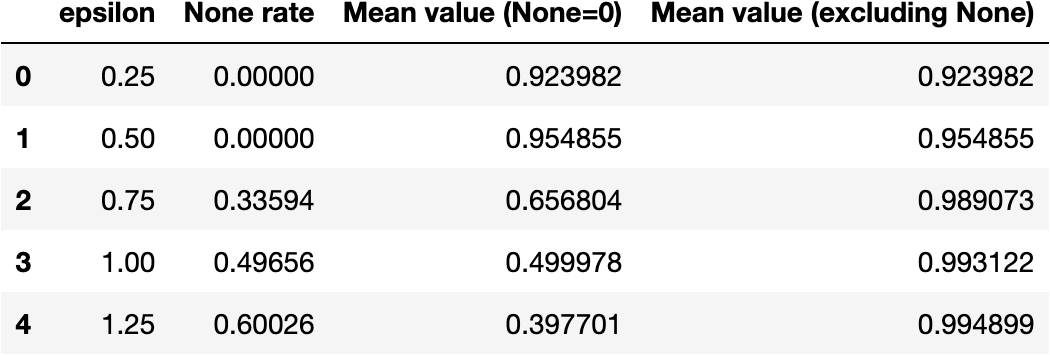
\includegraphics[width=\linewidth]{Images/extension/FairGeneralProphet_uniform_table.jpeg}
    \caption{uniform, performance metrics}
    \label{fig:extension_fairPA_uniform_table}
  \end{subfigure}
  \hfill
  \begin{subfigure}[t]{.5\textwidth}
    \centering
    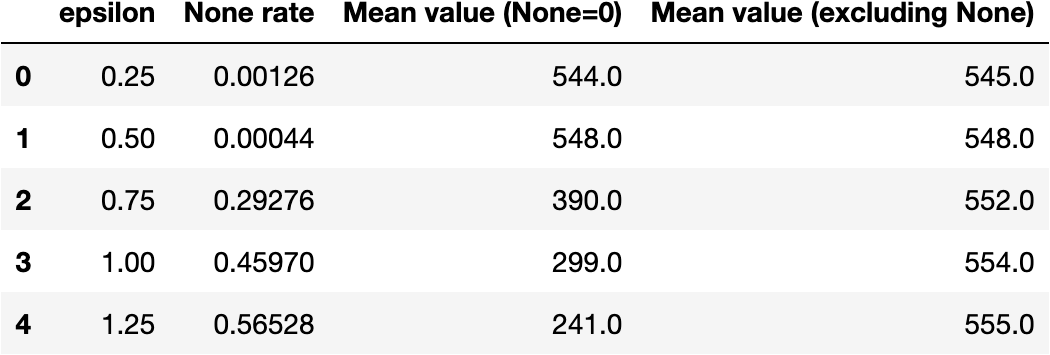
\includegraphics[width=\linewidth]{Images/extension/FairGeneralProphet_binomial_table.jpeg}
    \caption{binomial, performance metrics}
    \label{fig:extension_fairPA_binomial_table}
  \end{subfigure}

  \caption{
    Results grid search of FairPA, as presented in section \ref{sec:extension}. Figures \ref{fig:extension_fairPA_uniform} \& \ref{fig:extension_fairPA_binomial} show the number of picks per position for different values of $\epsilon$. The value $\epsilon = 1.0$ corresponds to the original paper's algorithm. Figures \ref{fig:extension_fairPA_uniform_table} \& \ref{fig:extension_fairPA_binomial_table} show None rates and mean scores (including and excluding None results) for both settings.
    }
\end{figure}



\begin{figure}[ht]
  \begin{subfigure}[t]{.5\textwidth}
    \centering
    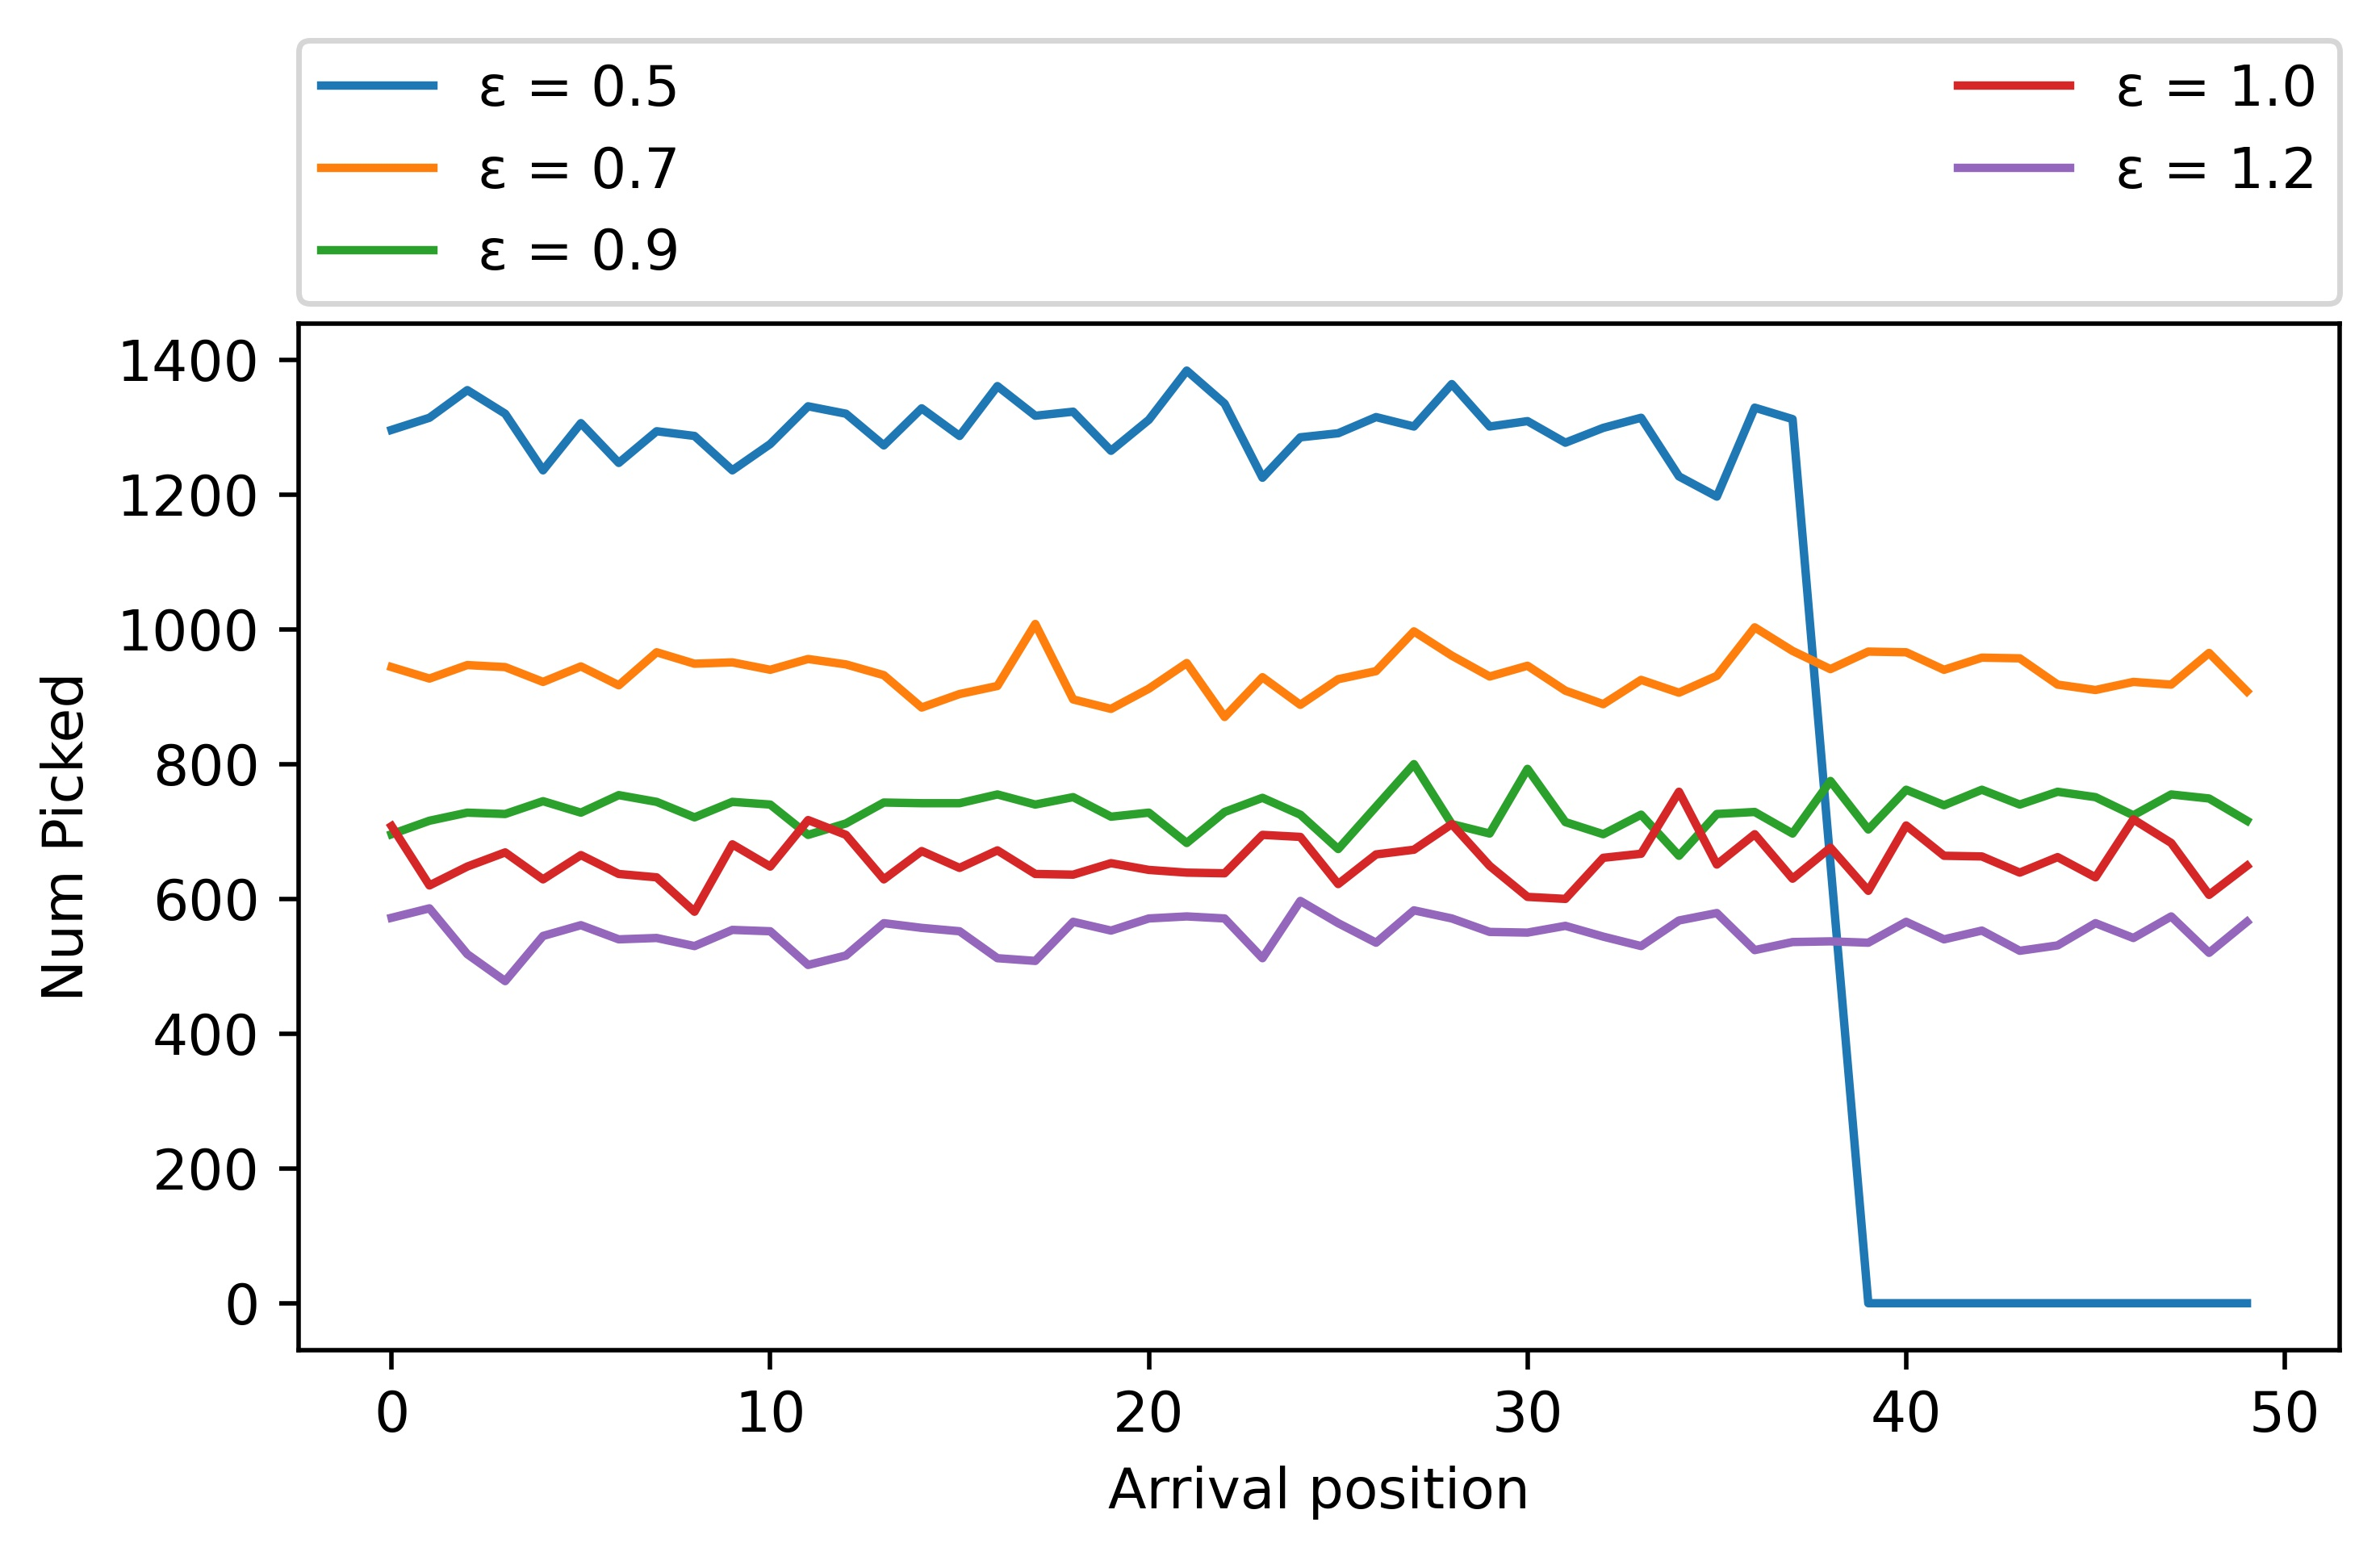
\includegraphics[width=\linewidth]{Images/extension/FairIIDProphet_uniform.jpeg}
    \caption{uniform}
    \label{fig:extension_fairIID_uniform}

  \end{subfigure}
  \hfill
  \begin{subfigure}[t]{.5\textwidth}
    \centering
    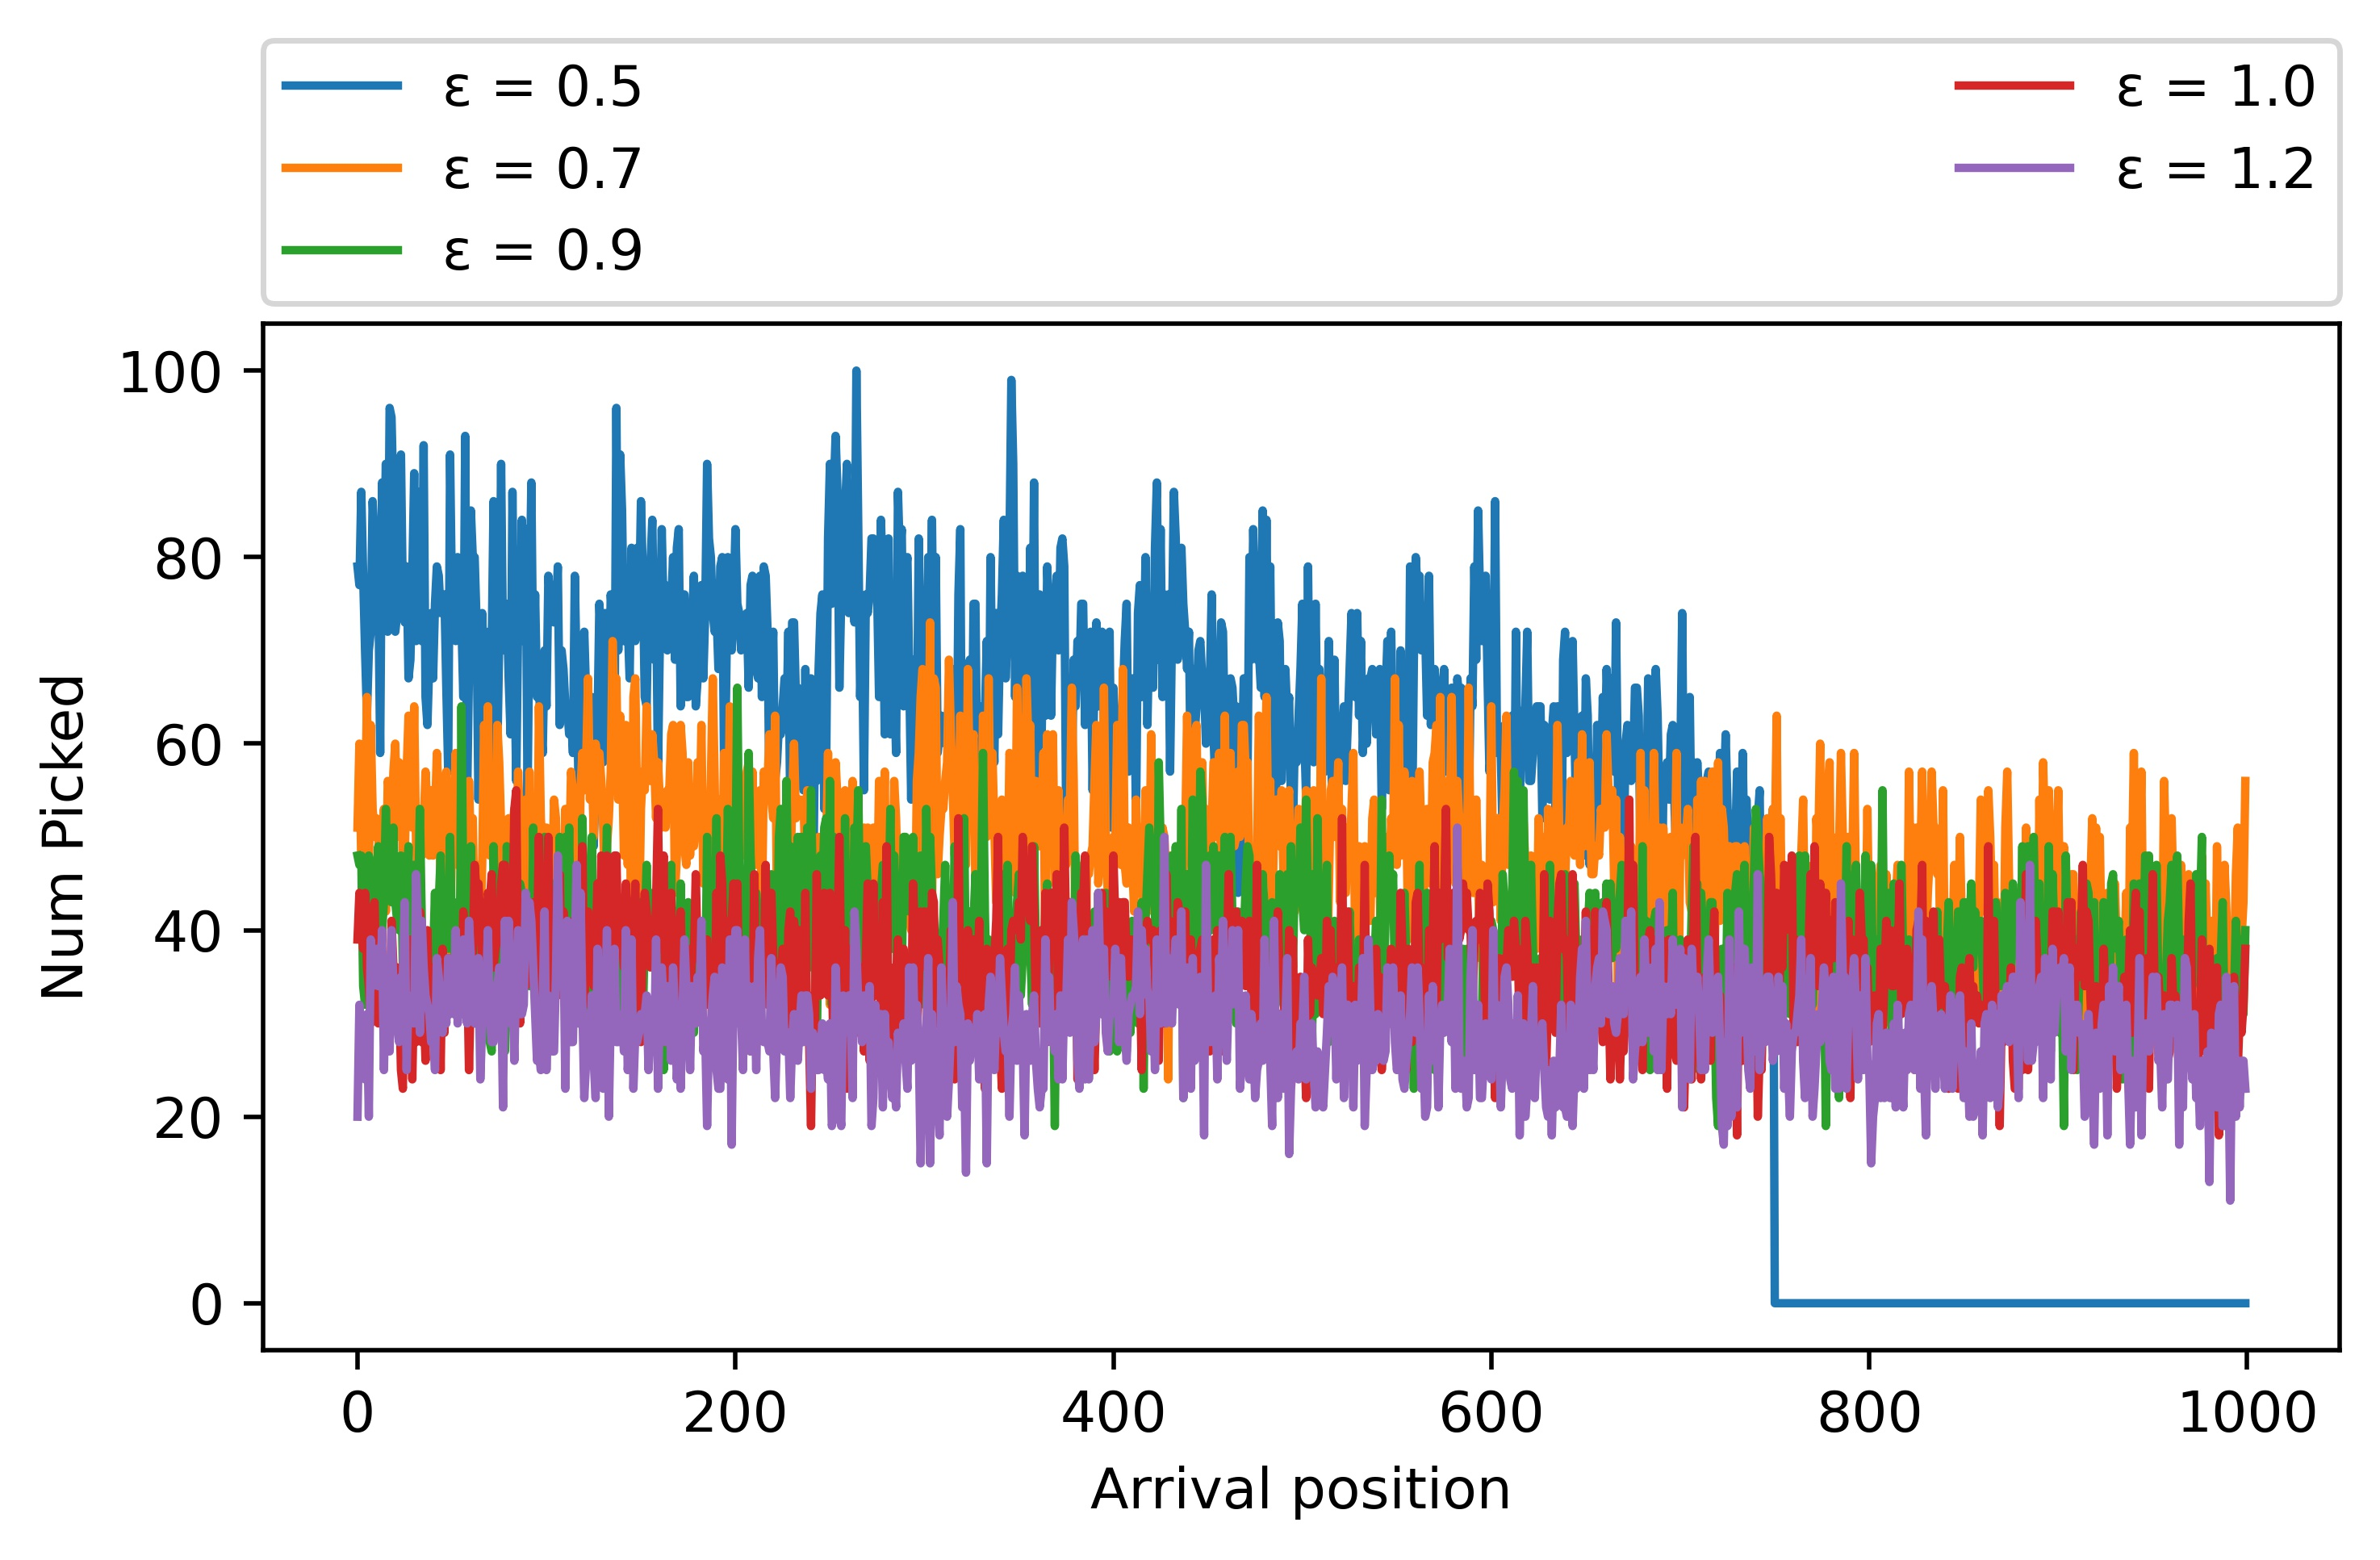
\includegraphics[width=\linewidth]{Images/extension/FairIIDProphet_binomial.jpeg}
    \caption{binomial}
    \label{fig:extension_fairIID_binomial}
  \end{subfigure}

  \medskip

  \begin{subfigure}[t]{.5\textwidth}
    \centering
    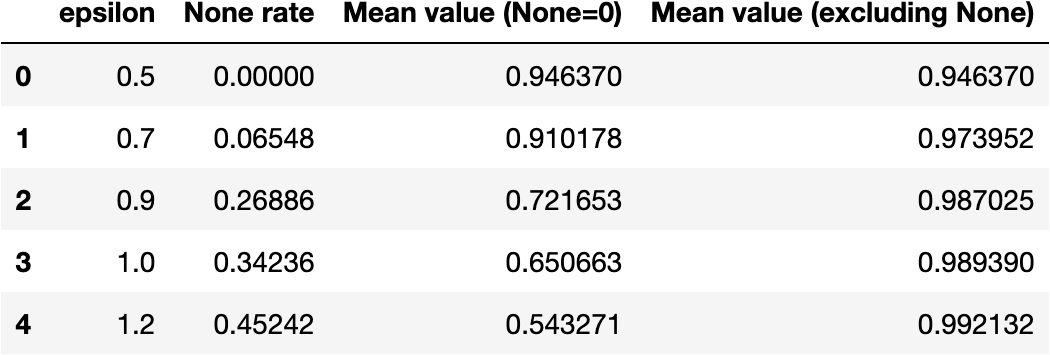
\includegraphics[width=\linewidth]{Images/extension/FairIIDProphet_uniform_table.jpeg}
    \caption{uniform, mean values}
    \label{fig:extension_fairIID_uniform_table}
  \end{subfigure}
  \hfill
  \begin{subfigure}[t]{.5\textwidth}
    \centering
    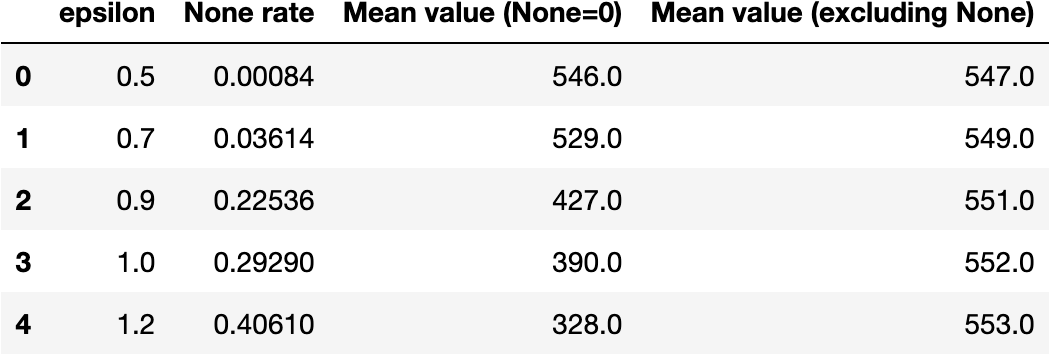
\includegraphics[width=\linewidth]{Images/extension/FairIIDProphet_binomial_table.jpeg}
    \caption{binomial, mean values}
    \label{fig:extension_fairIID_binomial_table}
  \end{subfigure}

  \caption{
  Results grid search of FairIID algorithm, as presented in section \ref{sec:extension}. Figures \ref{fig:extension_fairIID_uniform} \& \ref{fig:extension_fairIID_binomial} show the number of picks per position for different values of $\epsilon$. The value $\epsilon = 1.0$ corresponds to the original paper's algorithm. Figures \ref{fig:extension_fairIID_uniform_table} \& \ref{fig:extension_fairIID_binomial_table} show None rates and mean scores (including and excluding None results) for both settings.
  }
\end{figure}
